\documentclass[10pt]{article}

\usepackage{graphicx}
\usepackage{amsmath}
\usepackage[ansinew]{inputenc}
\usepackage[spanish]{babel}
\usepackage{babelbib}
\usepackage[T1]{fontenc}
\usepackage[vmargin=4cm,hmargin=4cm,letterpaper]{geometry}
\usepackage{color}
\usepackage{framed}
\usepackage{hyperref}

\usepackage{listings}
\definecolor{red}{RGB}{219,0,0}
\definecolor{pink}{RGB}{255,100,100}
\definecolor{gray}{RGB}{100,100,100}
\lstset{
		basicstyle=\ttfamily,
		frame=single,
		keywordstyle=\color{red},
		commentstyle=\color{gray},
		stringstyle=\color{pink},
		tabsize=3,
		language=verilog,
		backgroundcolor=\color{white}}

\usepackage{fancyhdr} 
\pagestyle{fancy}
\usepackage{lastpage}
\lhead{Laboratorio 2}
\chead{}
\rhead{Anteproyecto}
\lfoot{}
\cfoot{}
\rfoot{\footnotesize Page \thepage\ of \pageref{LastPage}}

\renewcommand{\headrulewidth}{0.4pt} 
\renewcommand{\footrulewidth}{0.4pt} 

\graphicspath{{./media/}}	%%multimedia path
\setlength{\parindent}{0pt}
%%*************************************************************************
\begin{document}

\begin{huge}
\begin{center}
\textbf{Laboratorio 2: Circuitos Combinatorios}
\end{center}
\end{huge}

\begin{Large}
\begin{center}
Jose Ap� (B10407), Francisco Molina (B12345), \\Marco Montero (A94000), Dennis Vargas (B16831)
\end{center}
\end{Large}


\section*{Objetivo General}
Utilizar el FPGA para el desarrollo de circuitos combinatorios.
\section*{Objetivos espec�ficos}
\begin{itemize}
\item Investigar el funcionamiento de la tarjeta de desarrollo FPGA Spartan 3E
\item Utilizar las herramientas del Xilinx ISE
\item Conocer y aplicar el flujo de dise�o para sistemas basados en FPGA
 \end{itemize}
 \section*{Problema}
 Agregue una operaci�n *MUL al experimento 1, esta operaci�n deber� multiplicar los valores de src1 y src2 y guardar el resultado en dst como se muestra a continuaci�n.
 \begin{table}[htdp]
\caption{default}
\begin{center}
\begin{tabular}{|c|c|c|c|c|}
\hline
Operacion & Destino & Fuente1 & Fuente2 & Descripcci�n \\
\hline
*MUL & dst & Src1 & Src2 & Dst = src1 * src2  \\
\hline
\end{tabular}
\end{center}
\label{default}
\end{table}%

\newpage
\section*{Ejercicio 1}
Agregue una operaci�n SMUL al experimento 1, esta operaci�n deber� multiplicar los valores de src1 y src2 y guardar el resultado en dst. \\ Antes de comenzar, anote la frecuencia que la herramienta de s�ntesis estima para el experimento 1, adem�s el n�mero de LUTs, Slices y Flip-Flops. Utilice el operador * de verilog para implementar la multiplicaci�n. \\ El Spartan 3E cuenta con bloques dedicados de multiplicaci�n. Por defecto, la herramienta de s�ntesis intentar� usar estos bloques dedicados de multiplicaci�n en lugar de sintetizarlos usando los bloques l�gicos de las celdas. Observe el reporte de la herramienta de s�ntesis. 
\begin{lstlisting}
========================================
Advanced HDL Synthesis Report
Macro Statistics
# RAMs : 2
 9x16-bit dual-port distributed RAM : 2
# ROMs : 1
 16x28-bit ROM : 1
# Multipliers : 1
 16x16-bit registered multiplier : 1
# Adders/Subtractors : 2
 16-bit adder : 2
 # Counters : 1
 16-bit up counter : 1
# Registers : 72
 Flip-Flops : 72
# Comparators : 1
 16-bit comparator lessequal : 1
========================================
\end{lstlisting}
\newpage
Los bloques de multiplicaci�n del FPGA son adem�s capaces de llevar acabo multiplicaci�nes con signo (con n�meros representados en complemento a 2). Para esto es
necesario que la herramienta de s�ntesis entienda que las lineas de entrada a los puertos del multiplicador tienen signo. \\Esto se hace de la siguiente manera:
\begin{lstlisting}
wire [9:0] wA, wB;
wire [31:0] R = wA * wB; //multiplicaci�n sin signo
wire signed [15:0] wA, wB;
wire signed [31:0] wR = wA * wB; // multiplicaci�n con signo
\end{lstlisting}
Note en la figura siguiente como el simulador reconoce la multiplicaci�n con signo:
\begin{figure}[hbtp]
\centering
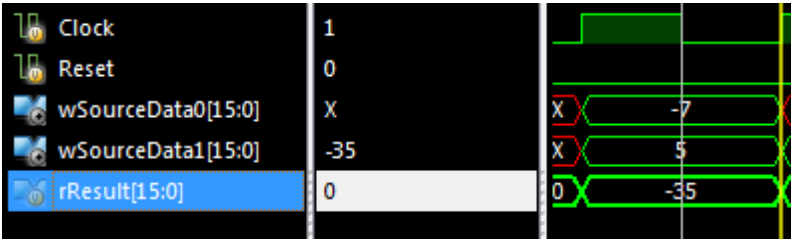
\includegraphics[width=12 cm]{media/r1.png}
\caption{}
\label{p1}
\end{figure}

Implemente la multiplicaci�n con signo usando el operador * de verilog. Anote la frecuencia que la herramienta de s�ntesis estima para esta parte, adem�s el
n�mero de LUTs, Slices y Flip-Flops. Modifique el c�digo en la ROM para calcular la multiplicaci�n de varios n�meros tanto con signo como sin signo y desplieguelo el resultado en los LEDs.

\subsection*{Soluci�n Propuesta}

\section*{Ejercicio 2}


\pagebreak 

\section*{Ejercicio 4}
Los warnings que s

\end{document}
%%*************************************************************************
